%!TEX root = ../thesis.tex
%*******************************************************************************
%****************************** Third Chapter **********************************
%*******************************************************************************
\chapter{Discussion}

% **************************** Define Graphics Path **************************

\graphicspath{{Chapter5/Figs/Vector/}{Chapter5/Figs/}}


\section{Non-Parametric}
Three algorithms tested of non-parametric variety producing several noticeable results. Firstly, the baseline result did not produce the worst results with respect to accuracy, although precision was consistently worse. This is demonstrated convincingly through Figure~\ref{fig:nPComp} where results from the greedy results suggest the worst accuracy.

Despite the greedy algorithm demonstrating the worst accuracy, interesting results were shown with ROD sampling. Indeed, the progression from the first to the second abd third iteration demonstrates a faster average learning rate than any other algorithm.

\begin{figure}[h]
    \begin{center}
        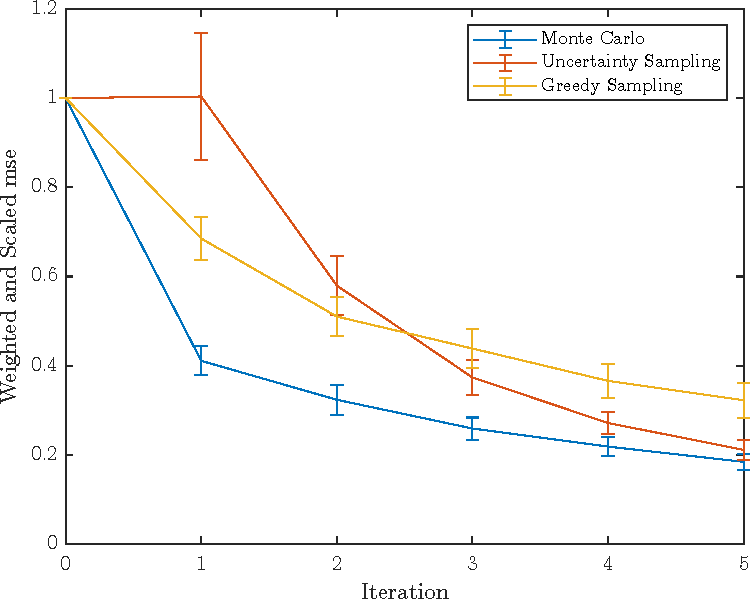
\includegraphics{nonParamComp1.pdf}
        \caption[Non-parametric comparison]{Comparison of different non-parametric algorithms with standard deviations represented as error bars.}
        \label{fig:nPComp}
    \end{center}
\end{figure}
\section{Parametric}
\blindtext[3]

